\chapter{State of the art}
\label{chap:stateoftheart}

\drop{T}{his} chapter aims to explain the concepts and techniques in which
Alcaudon is based on. As shown in Figure ~\ref{fig:mindmap}. the project has foundations in
distributed systems, job scheduling, library design and data processing. In the
next subsections, those concepts will be analyzed in more depth.

\begin{figure}[!h]
\begin{center}
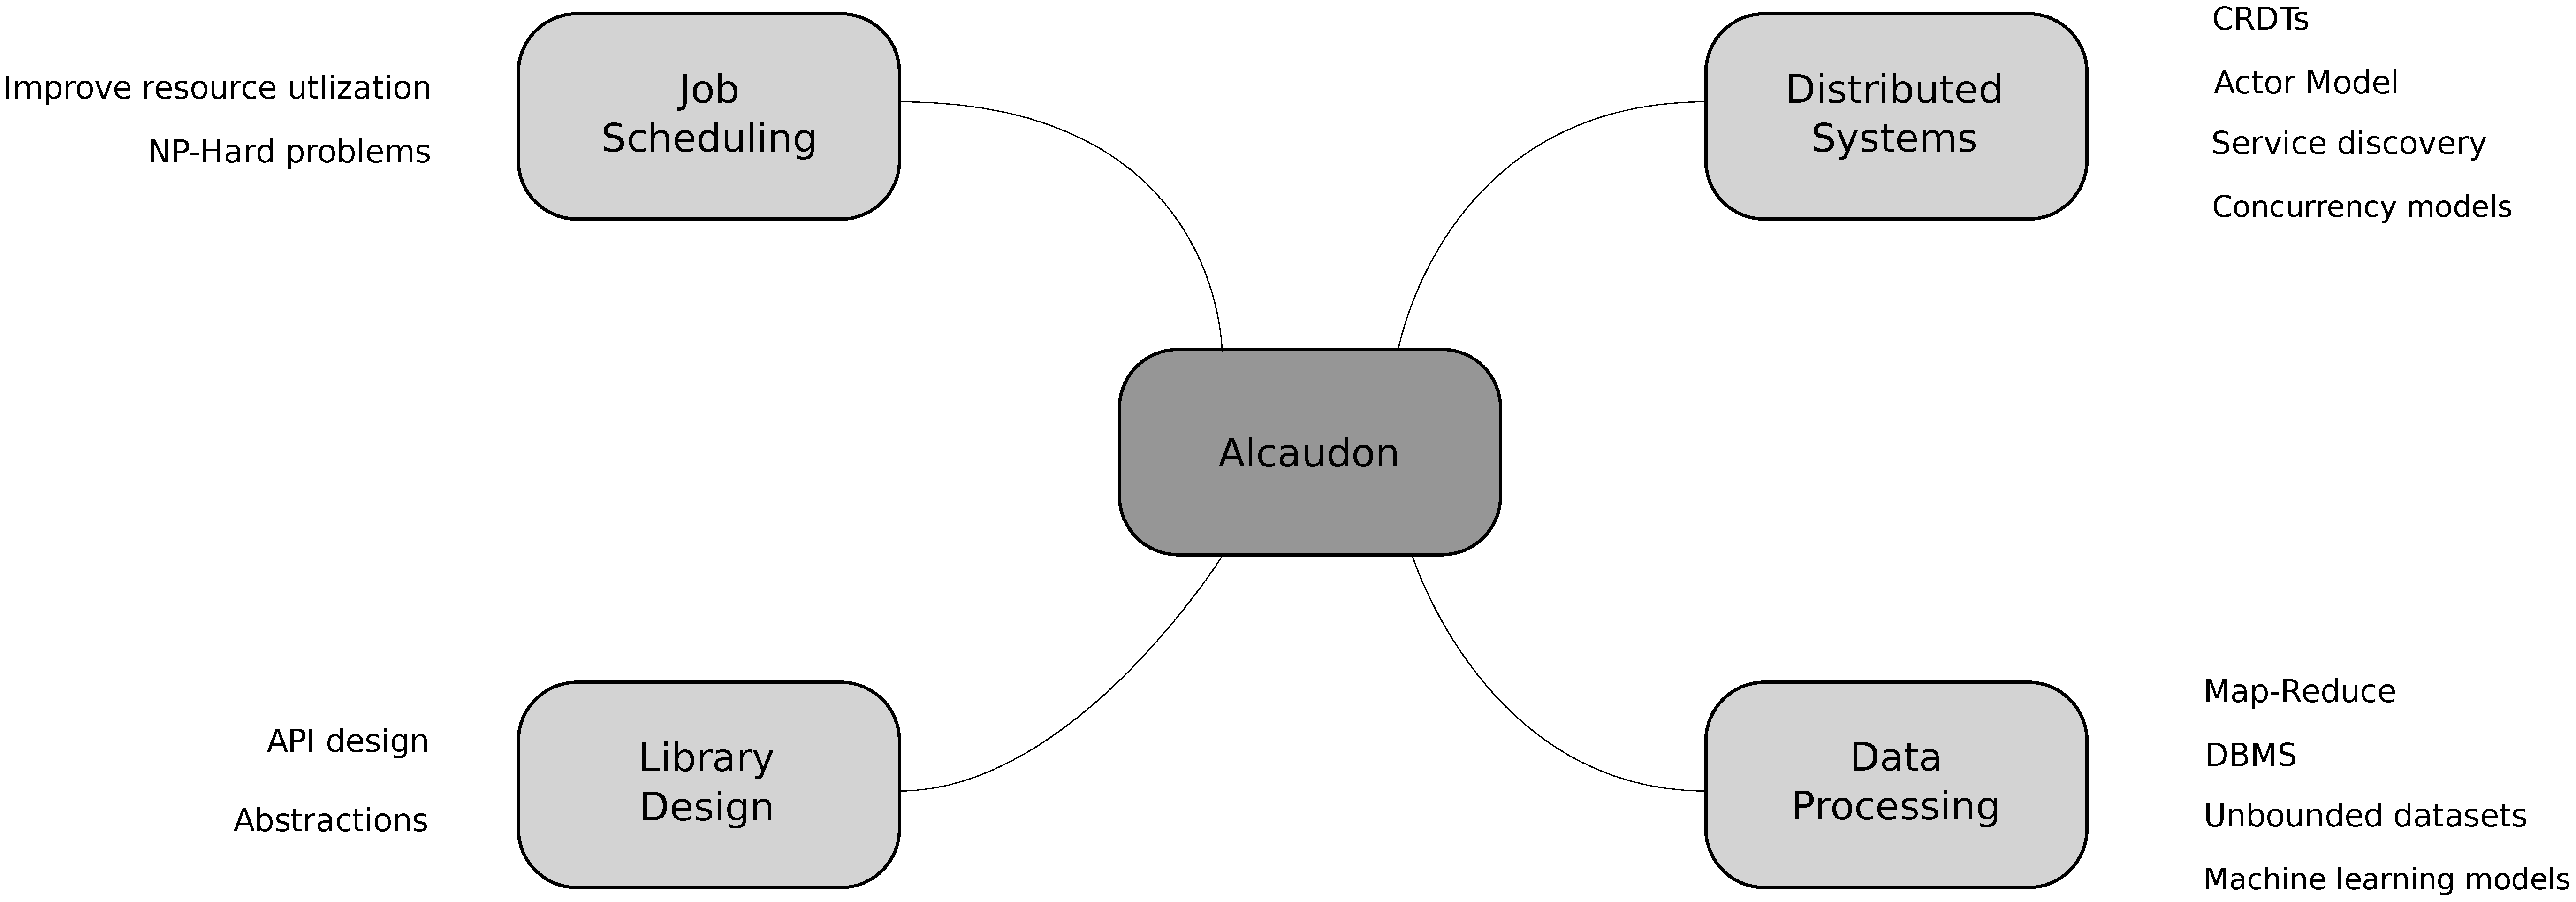
\includegraphics[width=1\textwidth]{mindmap.pdf}
\caption{Alcaudon foundations}
\label{fig:mindmap}
\end{center}
\end{figure}

\subsection{Data Processing}

According to a recent study by Cisco \cite{ciscosurvey}~\ref{fig:ciscodata} the
data storage is growing by 40\% yearly. This implies that that by 2020
datacenters will store over 1000 ExaBytes of information. Keeping that data in
silos without performing any use of it is a poor investment.

\begin{figure}[!h]
\begin{center}
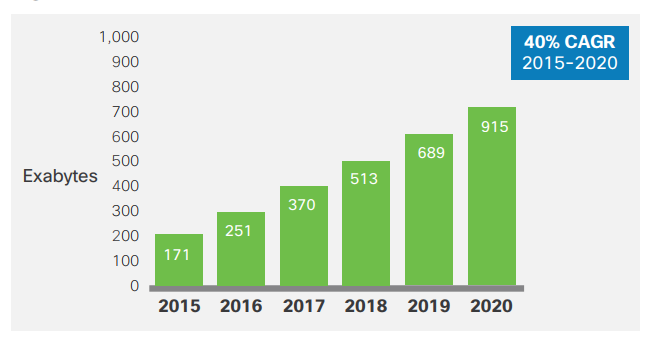
\includegraphics[width=0.8\textwidth]{ciscodata.png}
\caption{Actual Data Stored in Data Centers\cite{ciscosurvey}}
\label{fig:ciscodata}
\end{center}
\end{figure}

Processing those amounts of data using traditionals RDBMS is not practical, as they
are not designed to work with that much data. In the last years there have been
many ongoing efforts on providing tools to process and analyze large volumes of
data. Some examples could be MapReduce\cite{mapreduce}, Spark\cite{spark} and
many others. Before those frameworks appeared, there were some systems capable
of processing large amounts of data, like the supercomputers or HPC. One of the
main drawbacks of HPC is accessibility to those high end computers. Acquiring a
new Supercomputer in the event of a peak on data production is not feasible. For
companies, making an investment in a super computer is a big risk that in some
cases will not be reverted as profit. Another interesting point to make is that
Supercomputers perform well many floating-point operations per second. However,
in general, the computations executed in systems like MapReduce are simple
strings manipulation, counting and so on. Given these usage patterns, it seems
that supercomputers are more suited to perform scientific analysis.

Once the limitations of HPC for \textit{big data} scenarios have been described
it is possible to explore how modern internet companies are using computing
resources to process data. For new organizations, it is more sensible to take
advantage of commodity hardware to process large amounts of data. One of the
reasons is that there are many tools to distribute data processing among large
clusters of commodity machines. Once that job is done, those machines can be
turned off or used for other purposes. Working with those systems provides
flexibility, both in resource usage and innovation capacity. 

Even though systems such as Map-Reduce have been quite useful to process large
amounts of data, they start to have limitations in certain aspects. Currently,
the need of low latency in data processing is getting mandatory. Organizations
need to get insights about their data as soon as possible, in order to react
quickly to new trends. The systems described previously are classified as batch
systems, as they are oriented to process historical datasets and not
\textit{real time data}. There have been some adaptations to these systems, using
approaches like micro-batching where data is processed in smaller batches,
however the latency is still big. These new needs for data processing have lead
to the design and development of systems specialized in unbounded data
processing. These systems try to reduce the time between the event generation
and its processing. Alcaudon fits in this category of data processing systems,
as one of its aims is being able to process unbounded data sets with low
latency.

\subsubsection{Cloud Computing}

Cloud computing might be seen as a recent development. However, during the 1990s
researchers at Xerox PARC started to develop ideas around what they named
\textit{ubiquitous computing}. The idea was to have computing devices
interconnected and exchanging data about almost everything. This idea was ahead
of his time because there were just a few networks around. And devices such as
cameras and microphones were still quite big, etc. Even though if this definition is
translated to 2017 seems to fit quite perfectly on how devices behave nowadays.
Cars, fridges, watches, smartphones and anything that can have a network
interface is connected to the internet. Huge amounts of data are being published
and stored into the what is now known as \textit{the cloud}. There is not a
clear definition for what \textit{cloud computing} is. For the purposes of this
text, cloud computing could be defined as a pool of shared computing and storage
resources that can be provisioned and released on demand. Given the huge amounts
of data that users store into the \textit{cloud}, companies need to outsource
computing and storing capacity, since building datacenters is a huge investment.
In the last decade, computing infrastructure offering has changed radically.
Companies such as Amazon Web Services are able to offer servers, storage and
services on demand at scale, from 1 server to 1 million servers. Having the
ability to start and stop servers on demand has democratized the ability to
process large amounts of data for many organizations. For example, a startup can
kickoff with just one server to process data. Once the business starts growing,
it can take advantage of the elasticity provided by cloud computing services,
and start using more servers to cope with the load. This is one of the reasons why
data processing systems should be designed to scale out as there are more
computing needs.
Alcaudon, as an elastic data processing system, will be able to adapt to
different loads as the computing needs increase.. It will be able to use more
computing resources dynamically as more servers are added to the pool.

\subsection{Distributed systems}
\label{subsection:distsys}

Distributed systems can be defined as a set of computer programs, executing on
one or more computers, and coordinating actions by exchanging \textit{messages}
\cite{GuideReliable}. Those computers are usually located in a \textit{computer
  network}, a collection of computers interconnected by hardware that supports
message passing and implement routing protocols. But if this definition is taken
to the extreme, a modern multi-core processor can be characterized as a
distributed system, with many components exchanging information in a network and
coordinating actions to get work done. To some extent, it is possible to see
distributed systems as a super set of concurrent systems.

A more common example of a distributed system is a user requesting a web page to
a server with his smartphone. This example is a typical \textit{client-server}
model. This \textit{simple} action involves the interaction of various services
such as DNS servers, load balancers, HTTP proxies and HTTP servers. All these
services use a network as a mean to interchange messages as shown in figure
~\ref{fig:client-server}.

\begin{figure}[!h]
\begin{center}
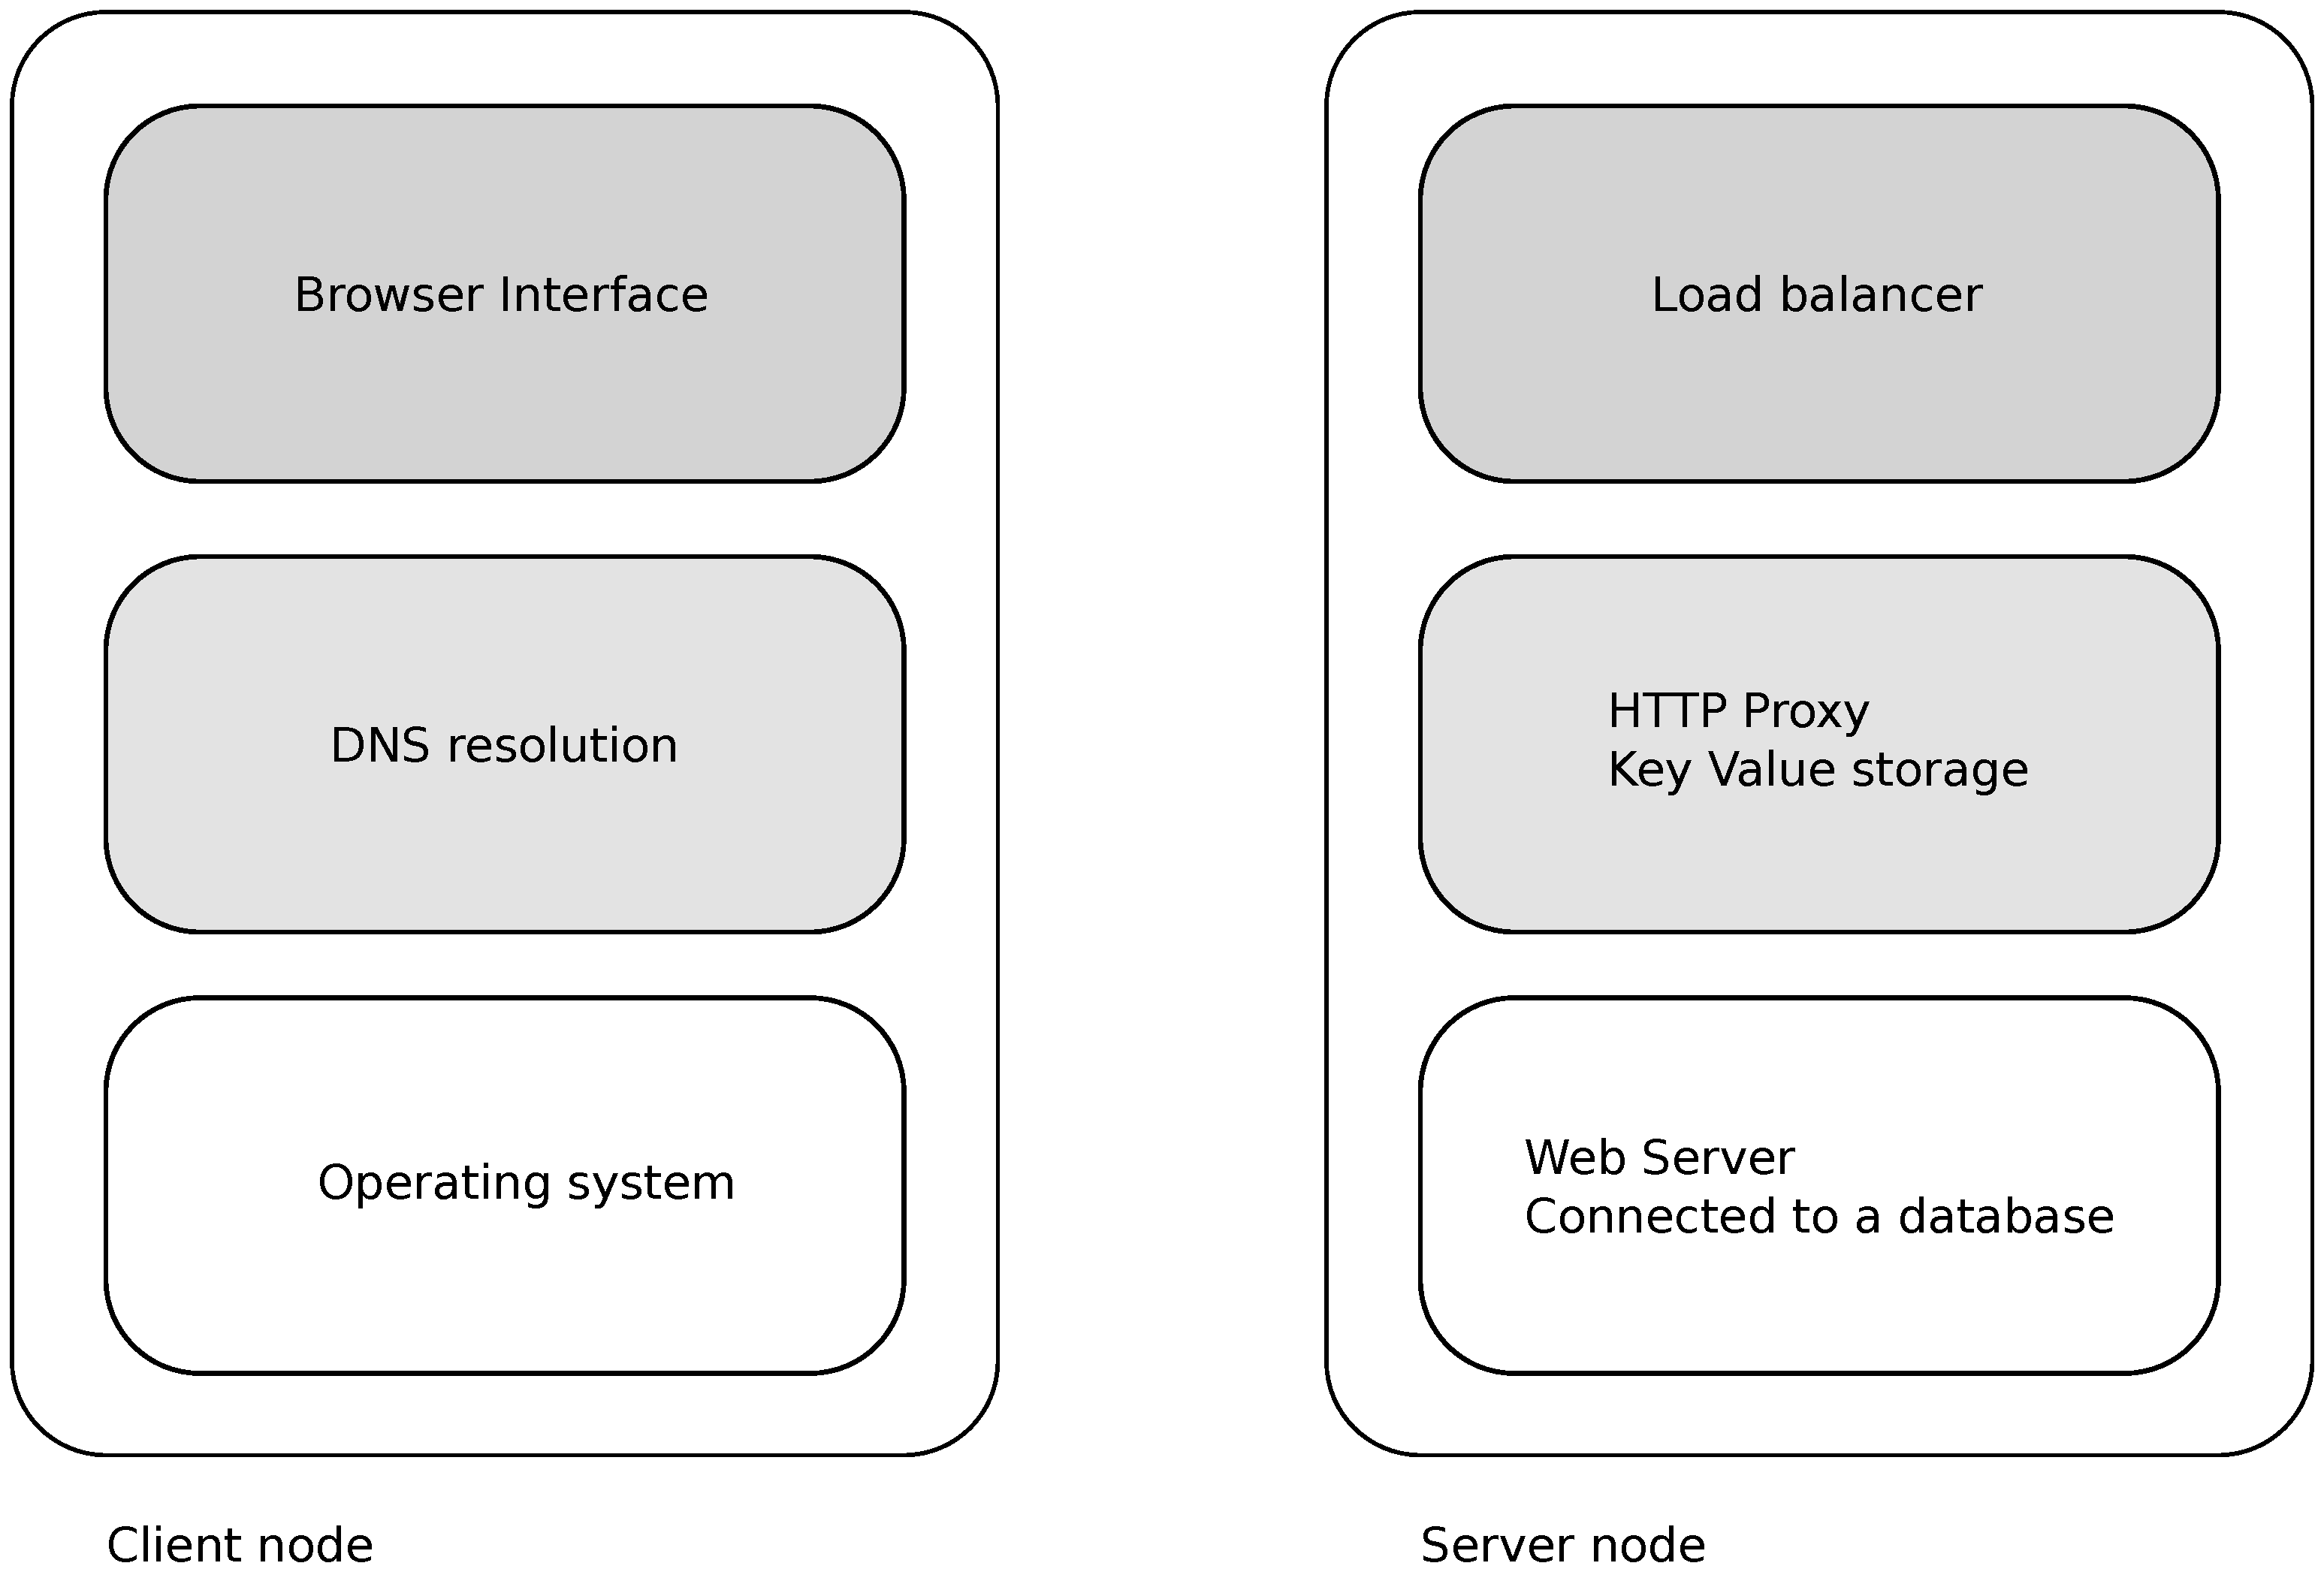
\includegraphics[width=0.7\textwidth]{client-server.pdf}
\caption{Client-server architecture}
\label{fig:client-server}
\end{center}
\end{figure}

As it has been previously discussed, distributed systems are very common
nowadays. They are present in fields like database systems, internet of things,
data processing and many more.

There are some reasons that make more convenient to work with distributed
systems, but the main reason is ability to scale. As defined in \cite{cloudadmin}
\begin{quote}
  A system's ability to scale is its ability to process a growing workload,
  usually measured in transactions per second, amount of data or number of
  users.
\end{quote}

Distributed programming can help designing systems with the ability to scale given
the following properties:

\begin{figure}[!h]
\begin{center}
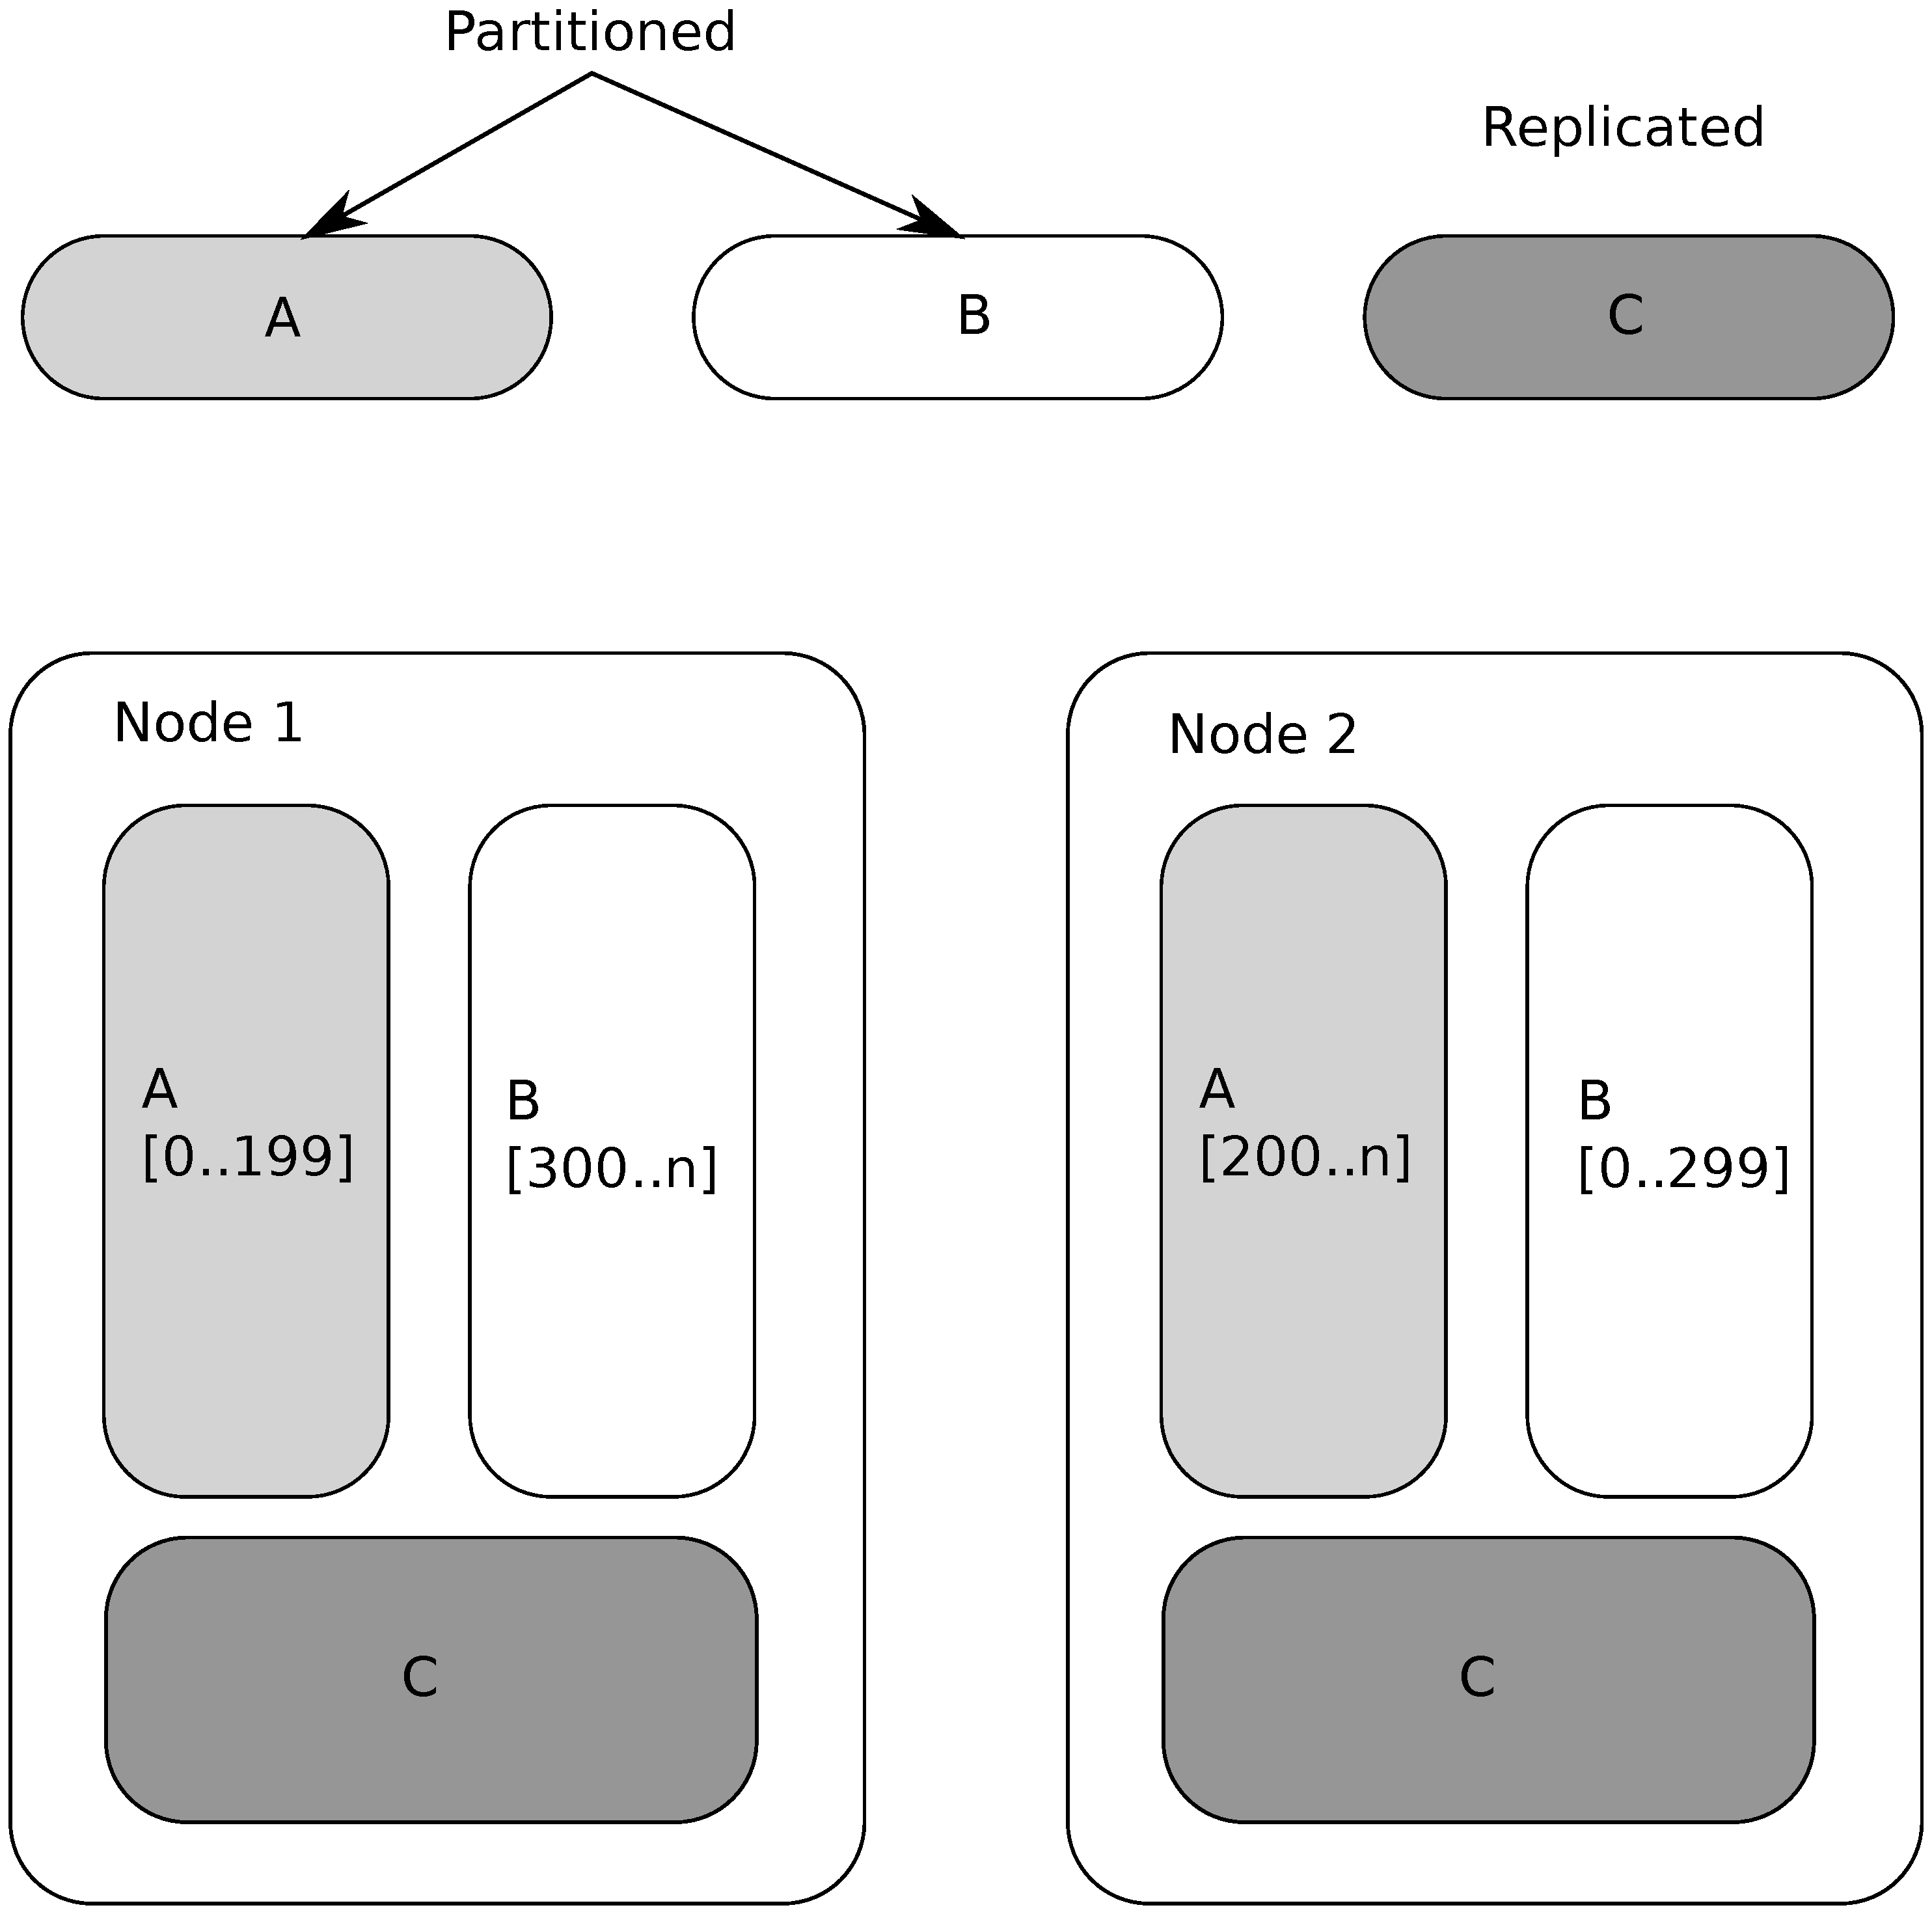
\includegraphics[width=0.7\textwidth]{partition-rep.pdf}
\caption{Partitioning and Replication}
\label{fig:partitioning}
\end{center}
\end{figure}

\begin{itemize}
\item \textit{Reliability}: Achieved by \textit{replication} and/or
  \textit{partitioning} as illustrated in Figure ~\ref{fig:partitioning}.
\item \textit{Elasticity}: Since the systems are designed to work in
  coordination with other processes, it is possible to add more resources to
  handle increasing workloads. But there is an upper limit imposed by the
  coordination model used.
\item \textit{Parallelism}: This is a natural outcome of having multiple resources, they
  can get work done in parallel.
\item \textit{Price/performance ratio}: Scaling vertically (using more powerful
  compute nodes), has upper limits both in available technology and in costs. As
  shown in Figure ~\ref{fig:highend} the performance gap between a high end
  server and a cluster of commodity hardware nodes is tolerable. Another factor
  to take into account when distributed systems are used is the cost of
  networking communications, as it implies an overhead in the computations.
\end{itemize}

\begin{figure}[!h]
\begin{center}
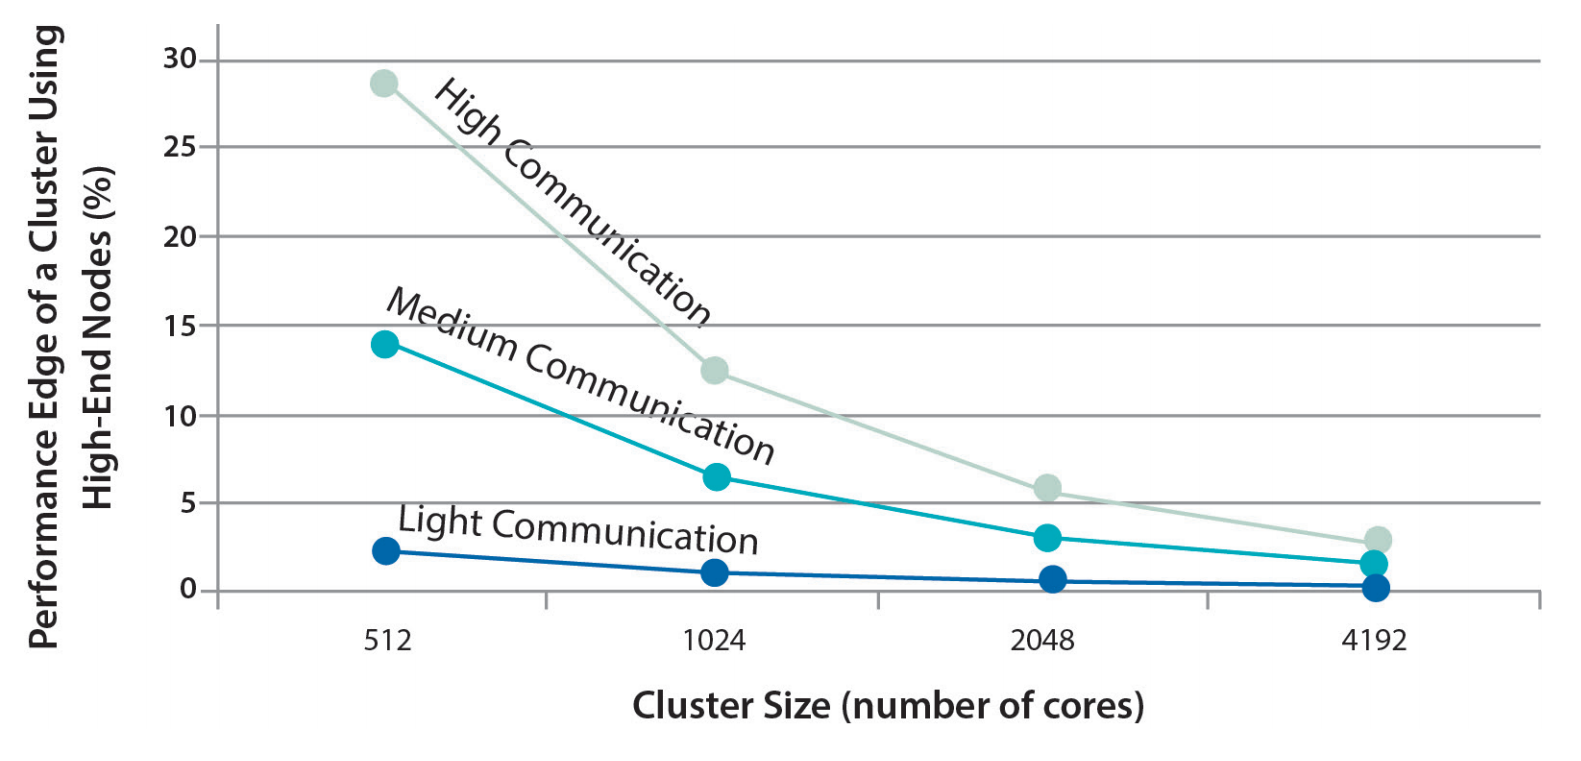
\includegraphics[width=1\textwidth]{scalingcost.png}
\caption{Performance advantage of a cluster built with large SMP server nodes
  (128-core SMP) over a cluster with the same number of processor cores built
  with low-end server nodes (four-core SMP), for clusters of varying
  size.\cite{Datacenter}}
\label{fig:highend}
\end{center}
\end{figure}

\subsubsection{Taxonomy of a distributed system}

Once described what distributed systems are and why they are useful, it is
possible to define a taxonomy of distributed systems topics such as coordination
algorithms, global state collection, distributed consensus, etc.

As it can be seen the topic is wide, so for this documents only
\textit{distributed snapshots}, \textit{membership protocols} and \textit{time
  in distributed systems} will be covered.

\begin{itemize}
\item \textit{Time in distributed systems}:
  Programmers are used to think in sequential programs, where computation steps
  are executed one after the other. The reality in distributed and concurrent
  systems is quite different. Knowledge about global state among all the nodes
  in the system is likely to be outdated. A naive solution to this problem is
  using synchronization based on wall clocks. However, the notion of
  synchronized clocks among nodes is impractical. Protocols like NTP\cite{ntp}
  can have skews up to 1000 seconds, an unacceptable time in some cases. Google
  makes heavy use of hardware-assisted time synchronization using GPS clocks and
  atomic clocks to ensure global consistency for their database
  Spanner\cite{180268} that can drift up to 100ms. Given the exposed facts, the
  only assumption that can be taken about global state that is partially
  ordered. A formal definition for partial order is \cite{book:lattices}:
\begin{definition}{Partial order}
  Let $P$ be a set. An order (or partial order) on $P$ is a binary relation
  $\leq$ on $P$ such that, for all $x$, $y$, $z \in P$,
  \begin{enumerate}
  \item $x \leq x$
  \item $x \leq y$ and $y \leq x$ imply $y$
  \item $x \leq y$ and $y \leq z$ imply $x \leq z$
  \end{enumerate}
\end{definition}
  Given the exposed facts, message order in distributed systems is partial. In
  environments where the message flow is unbounded the notion of completeness is
  weak. There is no guarantee about when all the messages up to a moment $T_n$
  have been received or processed. To deal with this, Alcaudon uses watermark
  heuristics. A watermark heuristic defines that up to the instant $T_i$ there
  are high chances that all messages up to that point have been received.
\item \textit{Distributed snapshots}:
  Since Alcaudon aims to be a fault-tolerant system, guarantees about persistent
  state must be enforced. To design a resilient system, persistent state
  snapshots should be taken. There are distributed algorithms to deal with this
  problem such as Lamport, bla, bla . In general, those algorithms are focused
  on taking a global state snapshot that given the constraints presented in the
  previous section is a hard problem to solve. In Alcaudon this obstacle is
  solved by taking snapshots by computation. There is no need of a global
  snapshot since persistent state is local to each computation.

\item \textit{Membership protocols}: Another crucial aspect on an elastic
  distributed system is how to handle cluster membership. It is possible to
  classify them into two categories: static membership and dynamic membership.
  Static membership has a fixed list of cluster members that do not change along
  the life of the cluster. With this static membership there is a chance that at
  some point in time, some members of the cluster will not be available. Since
  cluster membership image is static, thew will be seen as accessible. The other
  approach is to use dynamic membership. It consists on having initial knowledge
  about a subset of the available nodes and later on, via gossiping
  protocols\cite{gossip} new nodes can \textit{join} the cluster. This mechanism
  is also able to handle when nodes become \textit{unavailable}. For Alcaudon
  the latter membership category is more suitable. Since one of the goals is to
  provide elasticity, in this case the system will be able to be scaled in the
  need of more computing power.
\end{itemize}

\subsubsection{CRDT}

As previously presented, Alcaudon will be founded watermark heuristics. In order
to implement these heuristics, there is a need for some global knowledge about
latest processed events to keep track of the progress of ingested events into
the system. Each computation should be able to have partial knowledge of the
last watermark, and that depends on the state of a its dependencies. One of the
goals of the system is to avoid centralized coordination as much as possible, so
consensus based stores are discarded. One available option is Convergent
Replicated Data Types (CRDT)\cite{crdt}.


\begin{definition}{Merge properties}
  Let $P$ be a set. An order (or partial order) on $P$ is a binary relation
  $\leq$ on $P$ such that, for all $x$, $y$, $z \in P$,
  \begin{enumerate}
  \item $x \leq x$
  \item $x \leq y$ and $y \leq x$ imply $y$
  \item $x \leq y$ and $y \leq z$ imply $x \leq z$
  \end{enumerate}
\end{definition}

TODO


\subsubsection{Distributed system reliability}

Building distributed systems is not an easy task. In this subsection, different
failure scenarios that can happen in a distributed environment will be presented.

As proposed by \cite{GuideReliable}, it is possible to classify system error
causes as follows:
\begin{itemize}
\item \textit{Hardware failures}: These kind of failures are inevitable, since
  hardware has a life cycle and some components might fail or maintenance for
  components should be taken care of.
\item \textit{Software failures}: Software is becoming more and more complex.
  Software complexity errors such as coding errors, misguided software design,
  memory leaks or inadequate specifications are inevitable. There are countless
  examples of millionare losses, like when in 1999 NASA lost a Mars orbiter
  spacecraft because one team was working with Imperial units while another used
  metric units.
\item \textit{Complexity}: Developing software in distributed systems is
  complex. The notion of global state or order is fuzzy. Asynchronous
  communication is the norm. Regular developers are used to sequential
  computations, and getting familiarized to work within this environment is hard
  and can lead to bogus implementations. Luckily the use of formal verification
  is growing in the field, using tools such as TLA+\cite{tla} by Lamport. The
  usage of these techniques helps to tackle the inherent complexity with strong
  foundations.
\item \textit{Lack of failure detectors}: Most distributed systems try to detect
  failure just by using timeouts. This measure is quite straightforward to
  implement and reason about. The main drawback is that these techniques are
  raw. Vogels \cite{vogels} proposes a refinement over plain timeouts for
  failure detection, using more meta-information about the environment where
  the distributed system is running; reasoning about operating system metrics,
  networking metrics and disseminated probes, failure detection can improve.
\item \textit{Hostile environments}: There has been enumerated some reliability
  threats, which distributed systems need to deal with. Those threats are in
  \textit{control}, meaning that the developers of the system should anticipate
  them. Designing the systems so they are ready to deal with the exposed
  problems. However those systems run in shared networks where security threats
  are a reality. It is a wide field and it is becoming more and more important
  to take all the possible measures to avoid security vulnerabilities.
\end{itemize}

As a final note about other problems, there are costs associated with
distributed programming; network latency, fault-tolerance mechanisms and
consensus can have impact in the throughput achieved by a system. In
\cite{189908} a metric named Configuration that Outperforms a Single Thread
(COST), is proposed. It measures the number of cores needed to outperform a
single threaded implementation. In these experiments, there are many distributed
processing frameworks that don't perform properly when compared to single node
implementations. As a conclusion, there are scenarios where the costs associated
with distributed computing are higher than the gains.

Alcaudon's goal is to provide users a simple but powerful interface that enables
them to parallelize and distribute computations for unbounded datasets without all
the described problems.

\subsubsection{Actor Model}

To tackle all the complexity described in previous sections there is a
computation model that is well suited: the actor model.

The actor model provides a high level abstraction to deal with concurrent and
distributed systems. The theoretical model was developed by Carl Hewitt in
the seventies, but it was popularized by Erlang programming language\cite{erlang}
developed by Ericsson.

It can be characterized as follows:
\begin{itemize}
\item Actors communicate via asynchronous messages
\item Actors manage their state
\item In the event of a message response they can:
  \begin{itemize}
  \item Create new child actors
  \item Send messages to another actors
  \item Stop actors (even themselves)
  \item Change their behavior for the next messages
  \end{itemize}
\end{itemize}

Since distributed systems communicate asynchronously, this model fits perfectly,
because, even in single node environments, all the computations are executed in
response to asynchronous messages. The fact that the shared state among actors
is minimal helps to tackle all the inherent complexities around concurrency.
Another interesting outcome from designing the systems using message passing is
that creating protocols comes naturally in this model. The ability to change
their behavior depending on the incoming messages makes easy to model finite
state machines that fit perfectly with protocol design.

There are many implementations available\cite{wikiactor}, but the more popular
and stable versions are the Erlang programming language and Akka. Both versions
have similar features, in fact, Akka is highly inspired by Erlang. Nevertheless
Akka is built on top of the JVM, making it the most interesting implementation
available due to the vast ecosystem accessible around the JVM.

Akka has some extensions to the actor model that make it quite interesting to
build distributed systems.
\begin{itemize}
\item Actor supervision: One interesting approach of actor based design is how
  to handle failures. Each actor has a supervisor that handles its life-cycle,
  exceptions included. With this supervision schema it is easier to isolate failure
  scenarios into concrete actors instead of affecting the whole system. Each
  supervisor can define a strategy to apply when a child actor fails, i.e.
  restarting the actor or stopping it. This is highly beneficial because error
  handling logic is separated from business logic. These patterns resemble how
  ships are built, where the hull is compartmentalized into different watertight
  bulkheads. Therefore, if the hull is broken, the failure is limited to that
  bulkhead without compromising the ship stability. Alcaudon will benefit from
  this pattern to achieve fault-tolerant computations. One actor supervision
  tree can be found in figure~\ref{fig:supervision}.
\item Logical addresses: Each actor has a virtual address based on the actor
  system and its hierarchy. This helps providing location transparency, as
  actors can change their physical location and the framework will take care of
  routing messages to the new actor location.
\item Clustering: Support for distributed actors is provided, combined with
  logical addresses makes facilitates writing distributed applications.
\item Persistence: Akka supports actor state persistence. It is implemented as
  an append-only log. That technique is commonly used as transaction log in
  traditional databases, each change is appended to the transaction log. In case
  of a failure, those events are applied again to the in memory database
  buffers. To avoid long recovery times, snapshots from memory are taken
  regularly so the recovery process just needs to re-apply changes from that
  point. Akka persistence is implemented as described. This feature fits very
  well to mantain Alcaudon persistent state of computations, since computations
  can be defined as actors.
\end{itemize}

\begin{figure}[!h]
\begin{center}
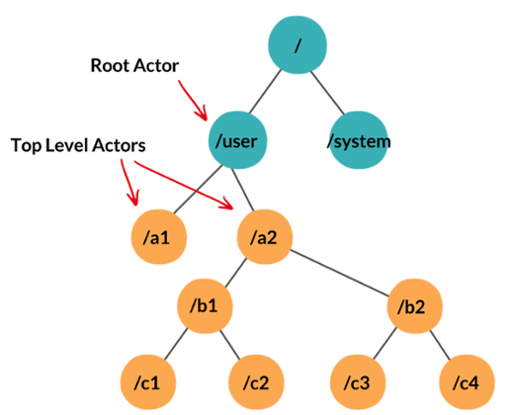
\includegraphics[width=0.8\textwidth]{supervision.png}
\caption{Actor supervision tree}
\label{fig:supervision}
\end{center}
\end{figure}

In conclusion, the actor model is a good computational model to base Alcaudon
on. It has properties that allows tackling all the presented difficulties around
writing distributed systems properly.

\subsection{Job scheduling}

Computations in distributed data processing clusters are expressed as a
dataflows. They can be considered as a direct acyclic graph (DAG) as the one in
Figure~\ref{fig:dataflow}.

\begin{figure}[h!]
\begin{center}
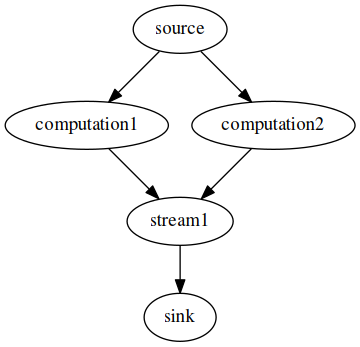
\includegraphics[width=0.6\textwidth]{dataflow.png}
\caption{Dataflow}
\label{fig:dataflow}
\end{center}
\end{figure}

One open problem in the construction of distributed data processing systems is
how to place those computations represented as a DAG, given a set of computing
nodes. This problem is known as the flexible Job-shop scheduling problem and it
has been widely studied during the last 60 years. One graphical example for $3$
jobs to be scheduled along $3$ machines can be seen in Figure~\ref{fig:jssp}.
As defined in\cite{jobshop2}:

\begin{definition}
In the flow shop scheduling problem we have a set of $n$ jobs that must be
processed on a given set of $m$ machines that are located in a fixed order. Each
job $j$ consists of a sequence of $m$ operations, where the $i$-th operation
must be processed during $p_{ij} \in \Z^{+}$ Time units without interruption on
the $i$-th machine. A feasible schedule is one in which each operation is
scheduled only after all operations preceding it in its job have been completed,
and each machine processes at most one operation at a time. A natural
generalization of the flow shop problem is to not require jobs to be processed
on all machines, i.e., a job still requests the machines in compliance with
their fixed order but may skip some of them. We will refer to this more general
version as generalized flow shops or flow shops with jumps. Generalized flow
shop (and thus flow shop) scheduling is a special case of the acyclic job shop
scheduling, which only requires that within each job all operations are
performed on different machines, which in turn is a special case of the general
job shop scheduling, where each job may have many operations on a single
machine. For any given schedule, let $C_j$ be the completion time of the last
operation of job $j$. We consider the natural and typically considered
objectives of minimizing the makespan, $C_{max} = max_j C_j$ , and the
\textit{sum of weighted completion times}, $\sum w_jC_j$ , where $w_j$ are
positive integers. The goal is to find a feasible schedule which minimizes the
considered objective function.
\end{definition}

\begin{figure}
\begin{center}
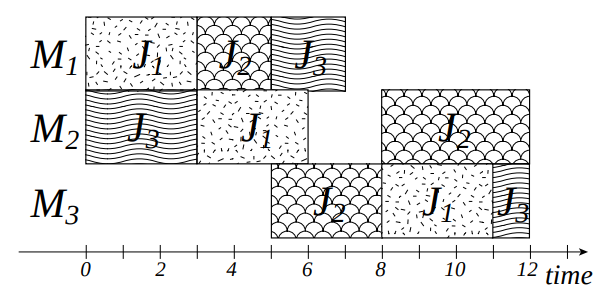
\includegraphics[width=0.6\textwidth]{jssp.png}
\caption{ A Gantt-Chart representation of a solution for a $3m \times 3j$ job scheduling problem\cite{geneticbook}}
\label{fig:jssp}
\end{center}
\end{figure}

Computing an optimal solution for this problem is a well known NP-hard
problem\cite{nphard}. Given this fact, all the proposed algorithms to solve this
problem are approximation algorithms. Some of the techniques used are listed
below:

\begin{itemize}
\item Algorithms based on priority rules and active schedule generation
\item \textit{Shifting bottleneck}
\item Simulated annealing
\item Tabu search
\item Genetic algorithms
\end{itemize}

How alcaudon solves this issue.

\subsection{Library design}

Humans have been using abstraction since the very beginnings of their existence.
The reality around is too complex to understand every detail of it. Thus,
abstraction is a really excellent tool to extract just the relevant facts about
the studied phenomenons. Computer Science, Software Engineering and Electrical
Engineering combine different abstractions in order to to build complex systems
in a manageable way.
Computer Science provides the tools whose roots are based on mathematical
foundations such as automaton theory, lambda calculus, language design, data
structures, etc.
Using those ideas, software engineering can be seen as the bridge between
hardware and computer science. It builds abstractions based on both worlds such
as operating systems, that hides the details of specific hardware and exposes an
uniform interface. And the list goes on. The main goal of abstractions is to
provide ways to reason about different problems with a limited scope.
As it has been exposed, providing tools that hide all the complexities is key to
build more complex systems. One of the main goals of the field since the late
60s has been to build reusable software\cite{reuse}. There have been many
advances in code reuse, from libraries and frameworks that are used to build
software on top them, to software as a service (SaaS). SaaS exposes public HTTP
API as the entry point to their functionality. This category of software reuse
can be the end of the spectrum, since the client just has knowledge about
the exposed interface and does not know anything about the underlying parts of the
system.

\begin{figure}[!h]
\begin{center}
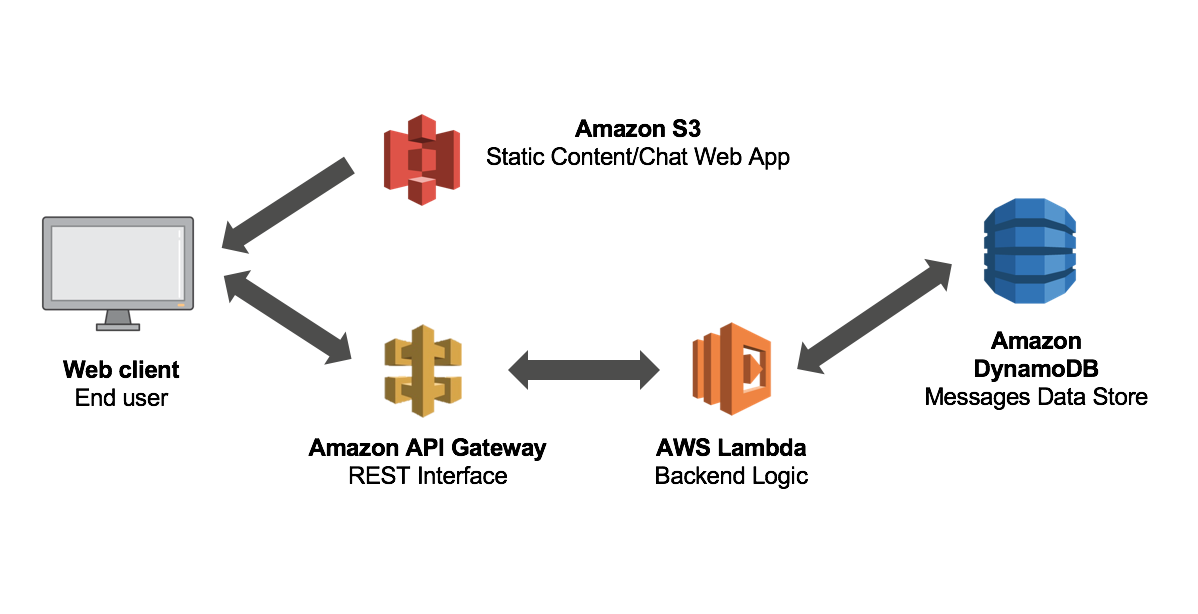
\includegraphics[width=0.8\textwidth]{serverless.png}
\caption{Serverless architecture example\cite{awsserverless}}
\label{fig:serverless}
\end{center}
\end{figure}

One recent trend in industry is serverless architecture like the one shown in
Figure~\ref{fig:serverless}. This programming model has foundations in reactive
programming, and it is based on providing code to produce computation results as
response to changes or events. In this paradigm it is just needed to provide
code implementing certain interface~\ref{code:lambdalisting} to handle events,
such as database changes, and the system will take care of deploy and run those
pieces together. As it can be observed, abstraction is going upwards and
programmers just need to take care of writing business logic and building
robust programs.

\begin{lstlisting}[language=java, frame=trBL, label=code:lambdalisting, float=ht, caption = {AWS Lambda Interface}]
  public interface RequestStreamHandler {
    public void handleRequest(InputStream inputStream, OutputStream outputStream, Context context)
    throws IOException
  }
\end{lstlisting}

Alcaudon philosophy is similar to the serverless architecture. The goal is to
provide abstractions around unbounded datasets so programmers just take care of
defining their computations and dependencies. Alcaudon will provide a simple
interface so the details to know about the system are minimized.
